\section{次微分}
\label{sec:ns-subdifferential}

函数在尖点没有导数，“导数为零”也就无从谈起。于是要问：在不可微的点，用什么量代替梯度，才能判断这个点是否最优？

\paragraph{尖点上的斜率}
先看$f(x)=\lvert x\rvert$。在$x\neq0$处，唯一的切线同时也是函数图像下方的一条支撑线。在$x=0$处没有切线，但有许多直线穿过原点且整条都不高于函数图像，也就是斜率$s$满足
\[
 \lvert y\rvert\geq s\,y\qquad\text{对所有}\ y.
\]

这个不等式对$s\in[-1,1]$成立，超出这个范围就会在某一侧穿到函数上方。图~\ref{fig:ns-support-lines}(a)画出了其中五条。

\begin{BookInlineFigure}
  \centering
  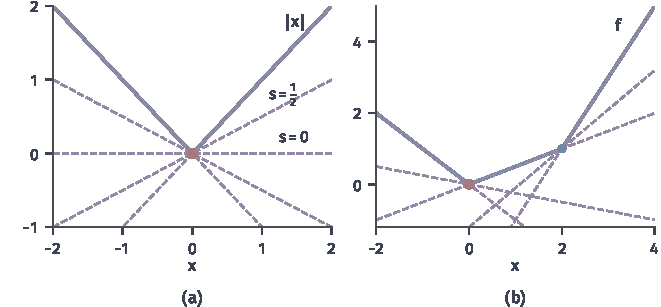
\includegraphics[width=112mm]{figures/05-optimization/03-nonsmooth-optimization/matplotlib/ns-support-lines/figure.pdf}
  \caption{尖点上的支撑直线。蓝线是函数，紫色虚线是不高于函数图像且在该点接触的直线，红点是最优解。(a)$\lvert x\rvert$在原点有斜率从$-1$到$1$的一整族支撑线，斜率$s=0$的水平线也在其中。(b)三段折线在$x=0$处的支撑斜率取遍$[-1,\tfrac12]$，在$x=2$处取遍$[\tfrac12,2]$，图中各画出几条。}
  \label{fig:ns-support-lines}
\end{BookInlineFigure}

可以把这些直线想成垫在碗底的一块木板。光滑的碗底只有一种放法，木板的倾角就是导数。碗底是尖的，木板可以在一定范围内摇摆，每个摆得开的倾角都是一条合格的支撑线。这个图景有一个边界：木板必须托住整个函数，不只是局部，所以下面的定义只适合凸函数。

\begin{definition}[次梯度与次微分]
\label{def:ns-subgradient}
设$f:\mathbb{R}^n\to\mathbb{R}\cup\{+\infty\}$是适当的凸函数，$\bm{x}\in\operatorname{dom}f$。若向量$\bm{g}\in\mathbb{R}^n$满足
\begin{equation}
 f(\bm{y})\geq f(\bm{x})+\langle\bm{g},\bm{y}-\bm{x}\rangle\qquad\text{对所有}\ \bm{y}\in\mathbb{R}^n,
 \label{eq:ns-subgradient}
\end{equation}
就称$\bm{g}$是$f$在$\bm{x}$处的\term{次梯度}（subgradient）。全体次梯度组成的集合
\begin{equation}
 \partial f(\bm{x})=\bigl\{\bm{g}:\ \bm{g}\ \text{满足式~\eqref{eq:ns-subgradient}}\bigr\}
 \label{eq:ns-subdifferential}
\end{equation}
称为$f$在$\bm{x}$处的\term{次微分}（subdifferential）。对$\bm{x}\notin\operatorname{dom}f$，规定$\partial f(\bm{x})=\varnothing$。
\end{definition}

式~\eqref{eq:ns-subgradient}的量词是“对所有$\bm{y}$”，这是全局信息。一元时它说的正是支撑线。多元时，右端是一个仿射函数的图像，也就是一张支撑超平面，它把函数的\term{上图}（epigraph）$\{(\bm{y},v):v\geq f(\bm{y})\}$整个留在上方。

次梯度与第~\ref{chap:optimization}章的梯度不是两种东西，可微点上它们重合。下面的定理同时说明，次微分什么时候确实存在。

\begin{theorem}[次微分的基本性质]
\label{thm:ns-subdiff-basic}
设$f$是适当的凸函数。
\begin{enumerate}
 \item $\partial f(\bm{x})$总是闭凸集（可能为空）。
 \item 若$f$在$\bm{x}\in\operatorname{int}\operatorname{dom}f$处可微，则$\partial f(\bm{x})=\{\nabla f(\bm{x})\}$。
 \item 若$\bm{x}\in\operatorname{int}\operatorname{dom}f$，则$\partial f(\bm{x})$非空且有界。
\end{enumerate}
\end{theorem}

\begin{proof}
第一条：每个固定的$\bm{y}$，把式~\eqref{eq:ns-subgradient}看成$\bm{g}$的条件，都给出一个闭半空间。$\partial f(\bm{x})$是这些闭半空间的交，所以是闭凸集。

第二条：设$\bm{g}\in\partial f(\bm{x})$，$\bm{d}$是任意方向。在式~\eqref{eq:ns-subgradient}中取$\bm{y}=\bm{x}+s\bm{d}$，$s>0$，得到
\[
 \frac{f(\bm{x}+s\bm{d})-f(\bm{x})}{s}\geq\langle\bm{g},\bm{d}\rangle.
\]

令$s\to0^+$，左端趋于$\langle\nabla f(\bm{x}),\bm{d}\rangle$，于是
\[
 \langle\nabla f(\bm{x})-\bm{g},\bm{d}\rangle\geq0\qquad\text{对所有}\ \bm{d}.
\]
取$\bm{d}=\bm{g}-\nabla f(\bm{x})$，只能有$\bm{g}=\nabla f(\bm{x})$。反过来，第~\ref{chap:optimization}章已经说明，凸函数的切平面是全局下界，所以$\nabla f(\bm{x})\in\partial f(\bm{x})$。

第三条的有界性：取$r>0$使闭球$\{\bm{y}:\lVert\bm{y}-\bm{x}\rVert_2\leq r\}$在$\operatorname{dom}f$内，凸函数在这个紧集上有上界$B$（把球放进一个小单纯形，函数值不超过顶点值的最大值）。对非零的$\bm{g}\in\partial f(\bm{x})$，取$\bm{y}=\bm{x}+r\bm{g}/\lVert\bm{g}\rVert_2$，由式~\eqref{eq:ns-subgradient}，
\[
 B\geq f(\bm{y})\geq f(\bm{x})+r\lVert\bm{g}\rVert_2.
\]
所以$\lVert\bm{g}\rVert_2\leq(B-f(\bm{x}))/r$。

第三条的非空性要用支撑超平面定理：上图是凸集，$(\bm{x},f(\bm{x}))$在它的边界上，过这一点存在一张支撑超平面。还需排除竖直的超平面，这一步由$\bm{x}$是内点保证。
\end{proof}

第三条非空性的详细论证可查阅\scite{rockafellar1970convex}。

边界点上次微分可以是空的。图~\ref{fig:ns-no-support}(a)的函数$f(x)=-\sqrt{x}$（$x\geq0$，其余为$+\infty$）是凸的，在$x=0$处切线竖直。任何有限斜率$s$的直线$sy$，在$y$足够小时都高于$-\sqrt{y}$，因为
\[
 -\sqrt{y}\geq s\,y\quad\Longleftrightarrow\quad\sqrt{y}\,(1+s\sqrt{y})\leq0,
\]
当$y\to0^+$时左端为正。所以$\partial f(0)=\varnothing$。第三条要求内点，正是为了排除这种情形。

\begin{BookInlineFigure}
  \centering
  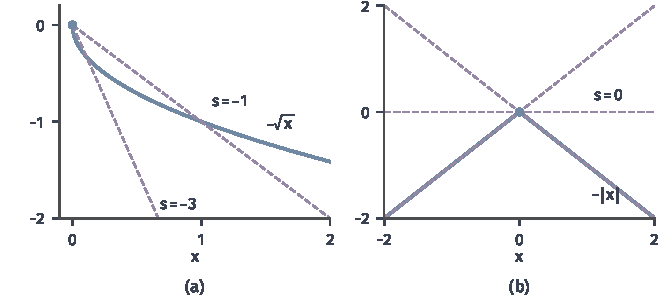
\includegraphics[width=112mm]{figures/05-optimization/03-nonsmooth-optimization/matplotlib/ns-no-support/figure.pdf}
  \caption{支撑线不存在的两种情形。(a)凸函数$-\sqrt{x}$在定义域端点切线竖直，紫色虚线（斜率$-1$和$-3$）在原点右侧贴近处都高出函数图像，所以次微分为空。(b)非凸函数$-\lvert x\rvert$的尖点朝上，任何穿过原点的直线都有一部分高于函数，按全局定义没有次梯度。}
  \label{fig:ns-no-support}
\end{BookInlineFigure}

\paragraph{几个计算}
绝对值的次微分由上面的讨论得到：
\begin{equation}
 \partial\lvert x\rvert=\begin{cases}\{\operatorname{sign}(x)\},&x\neq0,\\ [-1,1],&x=0.\end{cases}
 \label{eq:ns-abs-subdiff}
\end{equation}

坐标可分的函数$\sum_ic_i\lvert x_i\rvert$（$c_i>0$）的次微分是各坐标次微分的乘积。这是因为支撑不等式可以逐坐标相加，反过来只让一个坐标变化，就把每个坐标的不等式分离出来。

以菱形目标$f(\bm{x})=\lvert x_1\rvert+2\lvert x_2\rvert$为例，三个代表点的结果是
\[
 \partial f(0,0)=[-1,1]\times[-2,2],\quad
 \partial f(1,0)=\{1\}\times[-2,2],\quad
 \partial f(\tfrac12,\tfrac12)=\{(1,2)\}.
\]

图~\ref{fig:ns-diamond-subdiff}把点放在左边的$\bm{x}$平面，把次微分放在右边的斜率平面。越是“尖”的点，次微分越大：顶点处是长方形，棱上是线段，光滑的面内缩成一点。

\begin{BookInlineFigure}
  \centering
  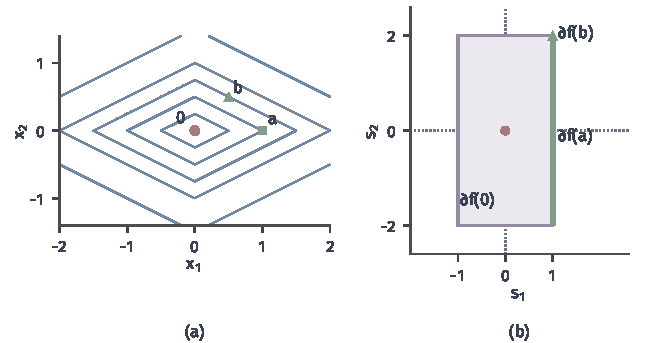
\includegraphics[width=112mm]{figures/05-optimization/03-nonsmooth-optimization/matplotlib/ns-diamond-subdiff/figure.pdf}
  \caption{菱形目标的次微分。(a)蓝线是$\lvert x_1\rvert+2\lvert x_2\rvert$的等高线，红点是最优解，$a=(1,0)$在棱上，$b=(\tfrac12,\tfrac12)$在光滑部分。(b)斜率平面：紫色长方形是原点的次微分，绿色粗线段是$a$处的次微分，绿色三角是$b$处的梯度。只有长方形包含$\bm{0}$（红点）。}
  \label{fig:ns-diamond-subdiff}
\end{BookInlineFigure}

有限个函数取最大值是尖点的另一个来源。最大值的尖点出现在分支交替的地方，这时次微分由活跃分支的梯度张成。把有限个向量的全部凸组合$\sum_i\theta_i\bm{g}_i$（$\theta_i\geq0$，$\sum_i\theta_i=1$）组成的集合称为它们的\term{凸包}（convex hull），记作$\operatorname{conv}$。

\begin{theorem}[有限最大值的次微分]
\label{thm:ns-max-subdiff}
设$f_1,\ldots,f_m:\mathbb{R}^n\to\mathbb{R}$都是可微的凸函数，$f=\max_if_i$，$I(\bm{x})=\{i:f_i(\bm{x})=f(\bm{x})\}$是活跃下标集。则
\begin{equation}
 \partial f(\bm{x})=\operatorname{conv}\bigl\{\nabla f_i(\bm{x}):\ i\in I(\bm{x})\bigr\}.
 \label{eq:ns-max-subdiff}
\end{equation}
\end{theorem}

\begin{proof}
记右端为$\bm{K}$。先证$\bm{K}\subseteq\partial f(\bm{x})$。对活跃的$i$和任意$\bm{y}$，
\[
 f(\bm{y})\geq f_i(\bm{y})\geq f_i(\bm{x})+\langle\nabla f_i(\bm{x}),\bm{y}-\bm{x}\rangle=f(\bm{x})+\langle\nabla f_i(\bm{x}),\bm{y}-\bm{x}\rangle.
\]
把这些不等式按$\theta_i$加权相加，就得到凸组合也满足式~\eqref{eq:ns-subgradient}。

再证反向。假设$\bm{g}\in\partial f(\bm{x})$但$\bm{g}\notin\bm{K}$。$\bm{K}$是紧凸集，可以严格分离：存在方向$\bm{d}$，使
\[
 \langle\bm{g},\bm{d}\rangle>\max_{i\in I(\bm{x})}\langle\nabla f_i(\bm{x}),\bm{d}\rangle.
\]

当$s>0$足够小时，不活跃的分支仍低于活跃分支，所以
\[
 f(\bm{x}+s\bm{d})=f(\bm{x})+s\max_{i\in I(\bm{x})}\langle\nabla f_i(\bm{x}),\bm{d}\rangle+o(s).
\]

另一方面，由式~\eqref{eq:ns-subgradient}，
\[
 f(\bm{x}+s\bm{d})\geq f(\bm{x})+s\langle\bm{g},\bm{d}\rangle.
\]
两式合起来除以$s$，令$s\to0^+$，与严格不等式矛盾。
\end{proof}

用这个定理算三段折线$f(x)=\max\{-x,x/2,2x-3\}$。三个分支的斜率是$-1,\tfrac12,2$。在$x=0$处前两支活跃，在$x=2$处后两支活跃，所以
\[
 \partial f(0)=[-1,\tfrac12],\qquad\partial f(2)=[\tfrac12,2].
\]

其余点只有一支活跃，次微分是单点。图~\ref{fig:ns-subdiff-graph}(b)把$\partial f(x)$画成$x$的集值图：普通的点对应水平线段上的一个值，尖点对应一条竖直线段，整条曲线是单调上升的台阶。单调上升这件事对应一元凸函数的导数非减。

\begin{BookInlineFigure}
  \centering
  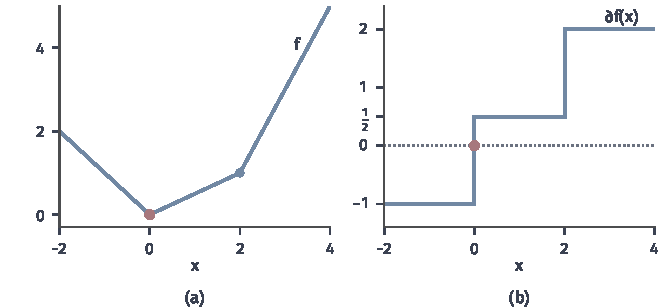
\includegraphics[width=112mm]{figures/05-optimization/03-nonsmooth-optimization/matplotlib/ns-subdiff-graph/figure.pdf}
  \caption{三段折线与它的次微分。(a)函数图像，红点是最优解。(b)次微分的集值图像，在两个折点处是竖直线段，点线是斜率为零的水平线。折线在$x=0$处的竖直线段穿过零，这就是最优性条件。}
  \label{fig:ns-subdiff-graph}
\end{BookInlineFigure}

\paragraph{最优性条件}
回到本节的问题。式~\eqref{eq:ns-subgradient}中令$\bm{g}=\bm{0}$，恰好读作“$f(\bm{y})\geq f(\bm{x})$对所有$\bm{y}$成立”。判据由此直接得到。

\begin{theorem}[凸目标的最优性条件]
\label{thm:ns-fermat}
设$f$是适当的凸函数，则
\begin{equation}
 \bm{x}^\star\in\argmin_{\bm{x}}f(\bm{x})\quad\Longleftrightarrow\quad\bm{0}\in\partial f(\bm{x}^\star).
 \label{eq:ns-fermat}
\end{equation}
\end{theorem}

\begin{proof}
由次梯度定义~\eqref{eq:ns-subgradient}，$\bm{0}\in\partial f(\bm{x}^\star)$与“对所有$\bm{y}$，$f(\bm{y})\geq f(\bm{x}^\star)$”是同一句话。
\end{proof}

这个判据比第~\ref{chap:optimization}章的一阶条件走得更远：它是充要的，而且结论是全局的，因为全局性已经写在定义里了。图~\ref{fig:ns-subdiff-graph}上读这个判据，就是找集值图穿过零线的地方。三段折线在$x=0$处$0\in[-1,\tfrac12]$，是最优解；在$x=2$处$0\notin[\tfrac12,2]$，不是。图~\ref{fig:ns-diamond-subdiff}(b)中，只有长方形包含原点。

\paragraph{和与复合的规则}
复杂的目标由简单的项拼成，希望次微分也能逐项计算。部分结论无条件成立，另一部分需要一个正则条件。下面用$\operatorname{ri}$表示\term{相对内部}（relative interior）：在集合自身张成的仿射子空间内的内点。若$\operatorname{dom}f$有内点，$\operatorname{ri}\operatorname{dom}f$就是内部。

\begin{theorem}[和与仿射复合]
\label{thm:ns-sum-rule}
设$f_1,f_2,f$是适当的凸函数，$\bm{A}\in\mathbb{R}^{p\times n}$，$\bm{c}\in\mathbb{R}^p$。对任意$\bm{x}$，
\begin{gather}
 \partial f_1(\bm{x})+\partial f_2(\bm{x})\subseteq\partial(f_1+f_2)(\bm{x}),\label{eq:ns-sum-inclusion}\\
 \bm{A}^\top\partial f(\bm{A}\bm{x}+\bm{c})\subseteq\partial\bigl(f(\bm{A}\,\cdot+\bm{c})\bigr)(\bm{x}).\label{eq:ns-affine-inclusion}
\end{gather}
若$\operatorname{ri}\operatorname{dom}f_1\cap\operatorname{ri}\operatorname{dom}f_2\neq\varnothing$，式~\eqref{eq:ns-sum-inclusion}取等号。若$\bm{A}$的值域经平移后与$\operatorname{ri}\operatorname{dom}f$相交，即存在$\bm{x}_0$使$\bm{A}\bm{x}_0+\bm{c}\in\operatorname{ri}\operatorname{dom}f$，式~\eqref{eq:ns-affine-inclusion}取等号。
\end{theorem}

\begin{proof}
两个包含关系只用定义。若$\bm{g}_i\in\partial f_i(\bm{x})$，把两条支撑不等式相加，就得到$\bm{g}_1+\bm{g}_2$是$f_1+f_2$的次梯度。若$\bm{g}\in\partial f(\bm{A}\bm{x}+\bm{c})$，对任意$\bm{y}$，
\[
 \begin{aligned}
 f(\bm{A}\bm{y}+\bm{c})&\geq f(\bm{A}\bm{x}+\bm{c})+\langle\bm{g},\bm{A}(\bm{y}-\bm{x})\rangle\\
 &=f(\bm{A}\bm{x}+\bm{c})+\langle\bm{A}^\top\bm{g},\bm{y}-\bm{x}\rangle.
 \end{aligned}
\]

反向的包含要由分离定理构造出分解，正则条件正是分离定理不退化所需要的，篇幅较长，可查阅凸分析的专著。
\end{proof}

下面的两个反例说明这些条件不能去掉。

先看和的反例。取$f_1(x)=-\sqrt{x}$（$x\geq0$，其余为$+\infty$），$f_2$是$(-\infty,0]$的约束指标函数。两者的有效定义域只在$0$处相交，相对内部$(0,\infty)$与$(-\infty,0)$不相交，条件不满足。$f_1+f_2$只在$0$处有限，所以
\[
 \partial(f_1+f_2)(0)=\mathbb{R},\qquad\partial f_1(0)+\partial f_2(0)=\varnothing.
\]
左边是整条实线，右边什么都没有，因为前面已经算出$\partial f_1(0)=\varnothing$。

再看复合的反例。取$f(u_1,u_2)=-\sqrt{u_2}$（$u_2\geq0$，其余为$+\infty$），$\bm{A}x=(x,0)$。值域是直线$u_2=0$，只碰到$\operatorname{dom}f$的边界。复合函数恒等于$0$，次微分是$\{0\}$，而$\partial f(x,0)=\varnothing$，等式同样失败。

实际中最常见的情形，至少有一项在全空间有限，比如$\lvert x\rvert$、$\lVert\bm{x}\rVert_1$和光滑项，正则条件自动成立。约束指标函数加有限函数也是如此，只要约束集非空。

外层是一元函数的复合还有一条常用规则：设$\psi:\mathbb{R}\to\mathbb{R}$是非减的凸函数，$c:\mathbb{R}^n\to\mathbb{R}$是可微的凸函数，则$\psi\circ c$是凸函数，且
\begin{equation}
 \partial(\psi\circ c)(\bm{x})=\bigl\{s\nabla c(\bm{x}):\ s\in\partial\psi(c(\bm{x}))\bigr\}.
 \label{eq:ns-monotone-chain}
\end{equation}

式~\eqref{eq:ns-monotone-chain}中“$\supseteq$”的方向可以直接验证。由$\psi$的支撑不等式和$s\geq0$（$\psi$非减保证了这一点），
\[
 \psi(c(\bm{y}))\geq\psi(c(\bm{x}))+s\bigl(c(\bm{y})-c(\bm{x})\bigr)\geq\psi(c(\bm{x}))+s\langle\nabla c(\bm{x}),\bm{y}-\bm{x}\rangle.
\]

第二步用到$s\geq0$和$c$的凸性。“$\subseteq$”的方向仍需要方向导数的论证。

例如$f(x)=\max\{0,x^2-1\}$，取$\psi=\max\{0,\cdot\}$，$c=x^2-1$。在$x=1$处，外层的次微分和内层的导数分别是
\[
 \partial\psi(0)=[0,1],\qquad c'(1)=2,
\]
于是$\partial f(1)=[0,2]$，这与函数左边斜率$0$、右边斜率$2$相符。若外层不单调，凸性本身就可能失败：$\lvert x^2-1\rvert$在$x=0$附近向下弯，式~\eqref{eq:ns-monotone-chain}不再适用。

\paragraph{贯穿例的最优性}
现在可以写出复合目标的最优性条件，并手工核验章首的问题。对
\begin{equation}
 F(\bm{x})=\frac12\lVert\bm{A}\bm{x}-\bm{b}\rVert_2^2+\lambda\lVert\bm{x}\rVert_1,\qquad\lambda>0,
 \label{eq:ns-lasso}
\end{equation}
这个问题常称为\term{Lasso}（least absolute shrinkage and selection operator）。两项都在全空间有限，和规则取等号。记$\bm{w}=\bm{A}^\top(\bm{A}\bm{x}-\bm{b})$，则$\bm{x}$最优当且仅当对每个坐标
\begin{equation}
 w_i=-\lambda\operatorname{sign}(x_i)\quad(x_i\neq0),\qquad\lvert w_i\rvert\leq\lambda\quad(x_i=0).
 \label{eq:ns-lasso-optimality}
\end{equation}

非零坐标上光滑项的梯度被绝对值的斜率恰好抵消；零坐标上梯度只要不超过$\lambda$，绝对值在零点的那一段斜率范围足以把它吸收，这个坐标便可以留在零。这就是Lasso产生零系数的机制。

验证例~\eqref{eq:ns-lasso-example}的候选解$\bm{x}^\star=(2,0)$。先算残差和梯度：
\[
 \bm{A}\bm{x}^\star-\bm{b}=(-1,0,1),\qquad\bm{w}=\bm{A}^\top(\bm{A}\bm{x}^\star-\bm{b})=(-1,0).
\]

第一坐标$x_1=2>0$，要求$w_1=-1$，成立。第二坐标$x_2=0$，要求$\lvert w_2\rvert\leq1$，成立。因此$\bm{x}^\star=(2,0)$是最优解，最优值为
\[
 F^\star=\frac12(1+0+1)+2=3.
\]

相对地，原点不是解：此处$\bm{w}=-\bm{A}^\top\bm{b}=(-5,-2)$，两个分量的绝对值都超过$1$。

约束问题也可以放进这个框架。设$\bm{C}$是非空闭凸集，$\iota_{\bm{C}}$是它的约束指标函数。按定义，$\bm{g}\in\partial\iota_{\bm{C}}(\bm{x})$（$\bm{x}\in\bm{C}$）当且仅当
\begin{equation}
 \langle\bm{g},\bm{y}-\bm{x}\rangle\leq0\qquad\text{对所有}\ \bm{y}\in\bm{C}.
 \label{eq:ns-normal-cone}
\end{equation}

满足这个不等式的向量组成$\bm{C}$在$\bm{x}$处的\term{法锥}（normal cone），记作$\bm{N}_{\bm{C}}(\bm{x})$。若$f$在全空间有限且凸，由定理~\ref{thm:ns-fermat}和和规则，$\bm{x}^\star$是约束问题的解当且仅当$\bm{0}\in\partial f(\bm{x}^\star)+\bm{N}_{\bm{C}}(\bm{x}^\star)$。例如在$[0,1]$上最小化$(x-3)^2/2$，解是边界点$x^\star=1$，此处$f'(1)=-2$，$\bm{N}(1)=[0,\infty)$，所以$0\in-2+[0,\infty)$。这个判据在第~\ref{chap:constrained-optimality}章会展开成乘子形式。

\paragraph{非凸函数的广义导数}
定义~\ref{def:ns-subgradient}依赖全局不等式，离开凸函数就不再合适。图~\ref{fig:ns-no-support}(b)的$-\lvert x\rvert$在原点按全局定义没有次梯度，但它是局部Lipschitz函数，尖点处的斜率信息是有意义的。常用的办法是只看局部，把附近可微点的梯度取极限。

对局部Lipschitz函数$f$，几乎处处可微，令$\bm{D}$为可微点集合，定义\term{Clarke次微分}（Clarke subdifferential）
\begin{equation}
 \partial_{\mathrm{C}}f(\bm{x})=\operatorname{conv}\Bigl\{\lim_{k\to\infty}\nabla f(\bm{x}^{(k)}):\ \bm{x}^{(k)}\to\bm{x},\ \bm{x}^{(k)}\in\bm{D}\Bigr\}.
 \label{eq:ns-clarke}
\end{equation}

这里的$(k)$是取极限用的序列编号。凸函数的Clarke次微分与$\partial f$相同；$f$连续可微时它就是$\{\nabla f\}$。对$-\lvert x\rvert$，$\partial_{\mathrm{C}}f(0)=[-1,1]$，包含$0$，但原点却是极大点。

可见$\bm{0}\in\partial_{\mathrm{C}}f(\bm{x})$只是局部最优的必要条件，与光滑非凸问题的“驻点”处于同一地位，不能得出全局或局部最优的结论\scite{math-clarke1990optimization}。本章其余部分遇到非凸目标时只用一种形式：$f$连续可微但可以非凸，$r$是凸函数，把$\nabla f(\bm{x})+\partial r(\bm{x})$作为$f+r$的广义次微分，$r$局部Lipschitz时它正是Clarke次微分。

\begin{BookInlineTable}
  \centering
  \small
  \begin{tabular}{@{}llll@{}}
    \toprule
    对象 & 判据 & 是否充分 & 结论范围\\
    \midrule
    光滑函数 & $\nabla f=\bm{0}$ & 否 & 局部最优的必要条件\\
    光滑凸函数 & $\nabla f=\bm{0}$ & 是 & 全局最优\\
    非光滑凸函数 & $\bm{0}\in\partial f$ & 是 & 全局最优\\
    局部Lipschitz函数 & $\bm{0}\in\partial_{\mathrm{C}}f$ & 否 & 局部最优的必要条件\\
    \bottomrule
  \end{tabular}
  \caption{不同函数类上的一阶判据。是否充分取决于凸性，与是否光滑无关。}
  \label{tab:ns-optimality}
\end{BookInlineTable}

表~\ref{tab:ns-optimality}汇总了这些判据。非光滑不会削弱判据的强度，凸性才决定“驻点”能否等于最优解。
